\section{Methods and results}

Our \ac{SVT} is built on top of 3D Slicer \cite{fedorov_3d_2012}.
3D Slicer, or simply `Slicer', is ``a free, open source and multi-platform software package widely used for medical, biomedical, and related imaging research''%
\fnurl{https://www.slicer.org/}.

We developed a Slicer module that leverages \ac{ITK} for image processing \cite{mccormick_itk_2014}, \ac{VTK} for visualization \cite{schroeder_visualization_2006} and Qt for the \ac{GUI}%
\fnurl{https://www.qt.io}.
The Python package used to query the \svtdatabase database, called \texttt{mega\_analysis}, can be installed with \ac{PIP}.
The code, written in Python 3, is available on GitHub%
\fnurl{\svtgithub}.
We have also developed an lite online version hosted on Binder \cite{bussonnier_binder_2018}, which does not require installation of 3D Slicer and can be accessed through a web browser%
\fnurl{https://mybinder.org/v2/gh/fepegar/SVT-web/HEAD?filepath=SVT-web.ipynb}.
Our \ac{SVT} can be used on all major platforms: Windows, Linux and macOS.

\begin{figure}
  \centering
  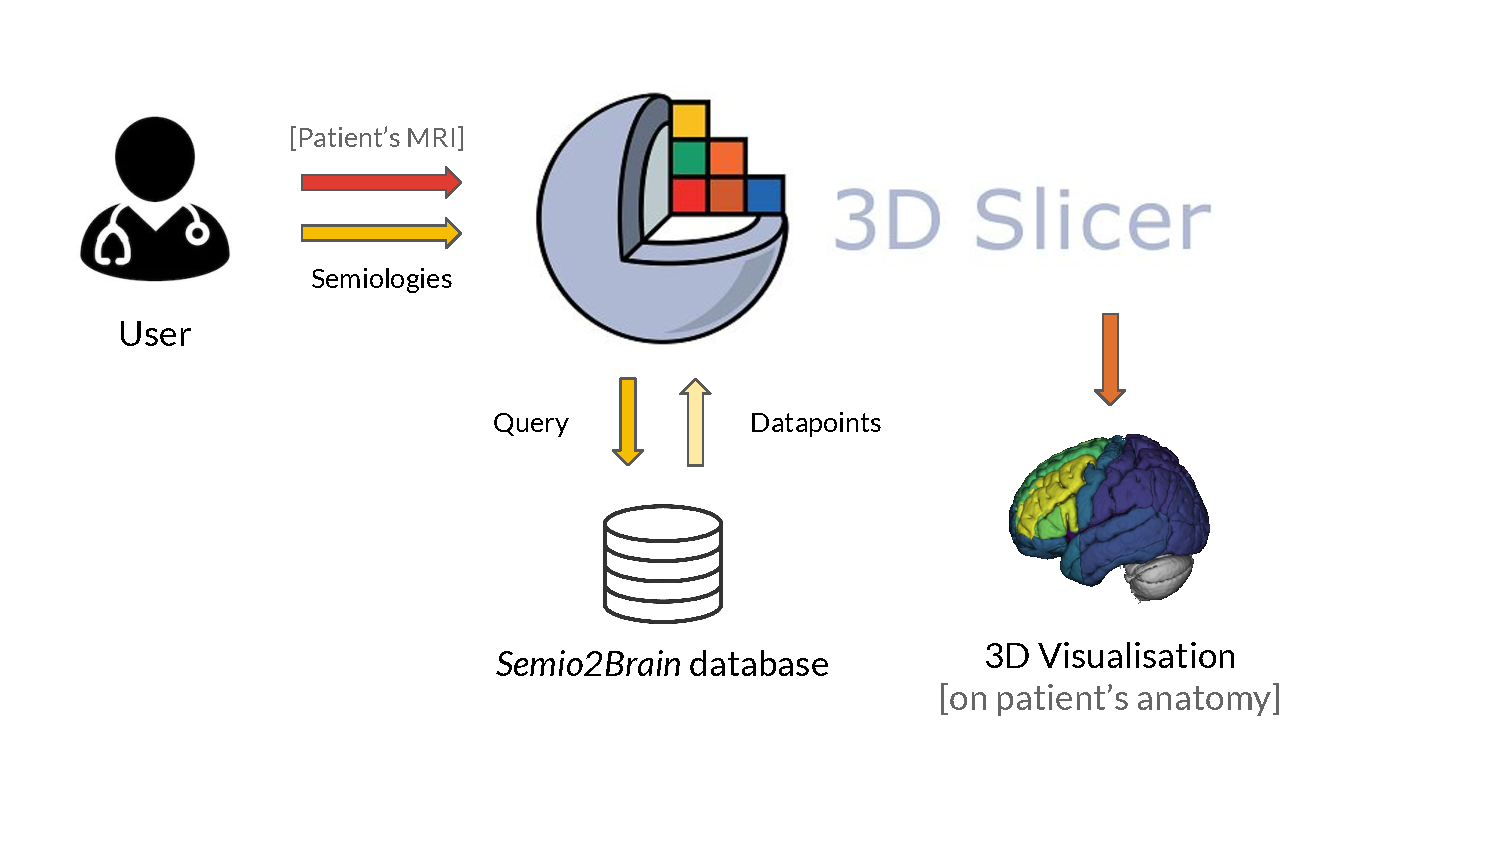
\includegraphics[trim=0 50 75 25, clip, width=\linewidth]{svt_2}
  \caption[General architecture of the Semiology Visualization Tool]{
    General architecture of the \ac{SVT}.
    The user inputs a list of observed seizure semiologies and (optionally) an \ac{MRI} of the patient for visualization in the patient's space.
    The \ac{GUI} is used to input the observed semiologies to the software, without the need to code.
    The Slicer module generates a structured query that can be processed by the \svtdatabase database querying module.
    The database is queried and the retrieved datapoints are converted into a \ac{3DMMI} visualization showing the \ac{EZ} probability map.
  }
  \label{fig:svt_architecture}
\end{figure}


\subsection{Data loading}

At start-up, the querying Python module is installed in the Slicer environment in the background, if it was not installed previously.

Then, the user is asked to load the patient's \ac{MRI} and a corresponding brain parcellation.
If the patient's data is not available or the \ac{SVT} is being used to explore the database and not for surgical planning, a generic \ac{MNI} template is loaded instead \cite{fonov_unbiased_2009}.
As the \ac{EZ} is expected to be in the gray matter, the parcellation is automatically stripped from the white matter and other irrelevant structures.
The expected brain parcellation must be compatible with the Neuromorphometrics atlas as it was used to build the \svtdatabase database.
However, the presented method is agnostic to the atlas choice.
All figures in this chapter show parcellations based on the Neuromorphometrics atlas, generated using \ac{GIF} \cite{cardoso_geodesic_2015}.
Finally, a Slicer segmentation node is instantiated from the parcellation label map, 3D meshes are generated for visualization using the marching cubes algorithm \cite{lorensen_marching_1987,pinter_polymorph_2019} and the user is presented with the preprocessed data (\cref{fig:svt_loaded}).

\newcommand{\svtscreenshot}[1]{
  \includegraphics[trim=0 65 0 47, clip, width=\linewidth]{#1}
}

\begin{figure}
  \centering
  \svtscreenshot{svt_loaded}
  \caption[Semiology visualization module after loading a patient's data]{
    Semiology visualization module after loading an \ac{MNI} template as image reference (as opposed to a patient's data) and its corresponding brain parcellation.
    Left: main panel containing a list of suggested semiology terms to be selected by the user;
    right: neuroimages in the patient's space.
    Images are shown using the radiological convention, i.e., the left hemisphere is shown on the right and vice versa.
  }
  \label{fig:svt_loaded}
\end{figure}


\subsection{Semiologies}

Once the data have been loaded, a pre-defined list of common semiologies is shown on the left-hand side of the screen (\cref{fig:svt_semiologies}).
Certain semiologies such as \textit{Head version} require a laterality (left or right).
Semiologies such as \textit{Hypermotor} may not have an associated laterality, meaning it was observed for both sides.
Some lateralities such as \textit{Ictal speech} never have an associated laterality.
The dominant hemisphere may also be specified, if known.
Custom semiologies may also be entered, which may be matched to one of the pre-defined semiologies using regular expressions \cite{alim-marvasti_mapping_2021}.
Matching is performed in real time every time the characters in the widget are modified, as long as at least three characters have been typed (\cref{fig:svt_custom}).

\begin{figure}
  \centering
  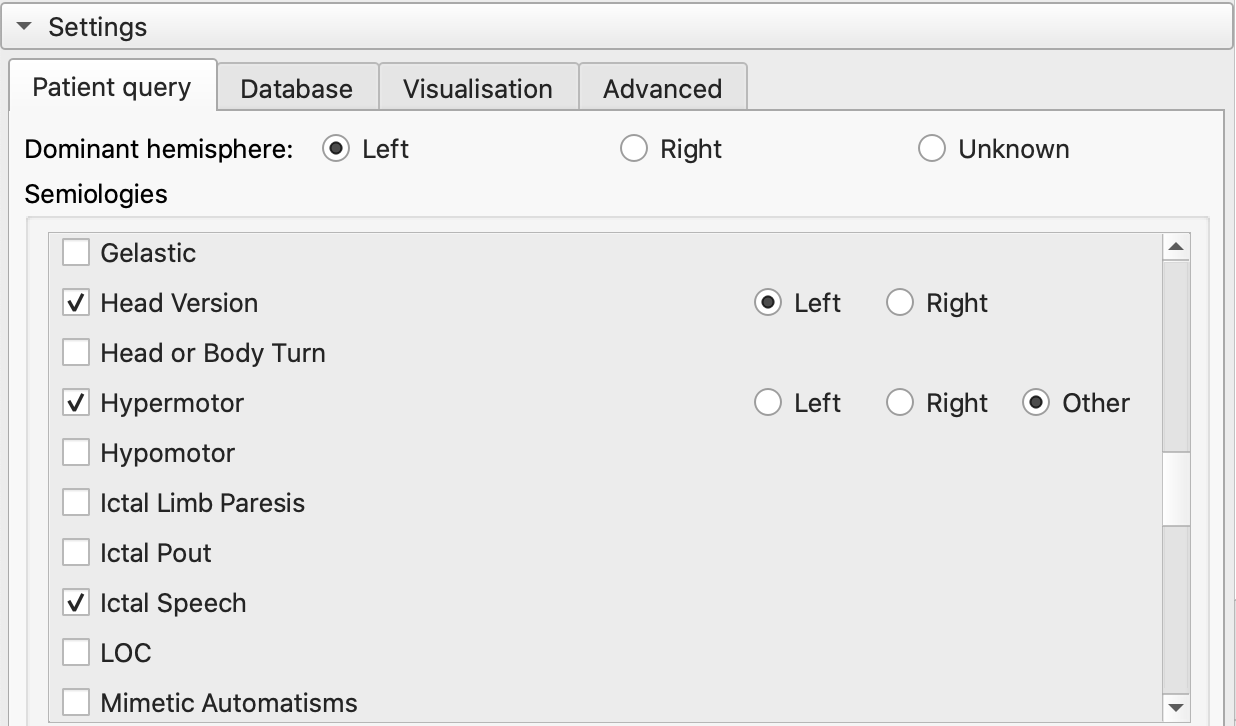
\includegraphics[width=\linewidth]{svt_semiologies}
  \caption[List of pre-defined semiologies in the GUI]{
    List of pre-defined semiologies in the \ac{GUI}.
    Users can select a semiology in the list or add a custom one, which might be matched to a pre-defined semiology using regular expressions to match concepts associated to that semiology.
    For example, `butterflies' and `déjà vu' would be matched with epigrastric and psychic auras, respectively.
  }
  \label{fig:svt_semiologies}
\end{figure}

\begin{figure}
  \centering
  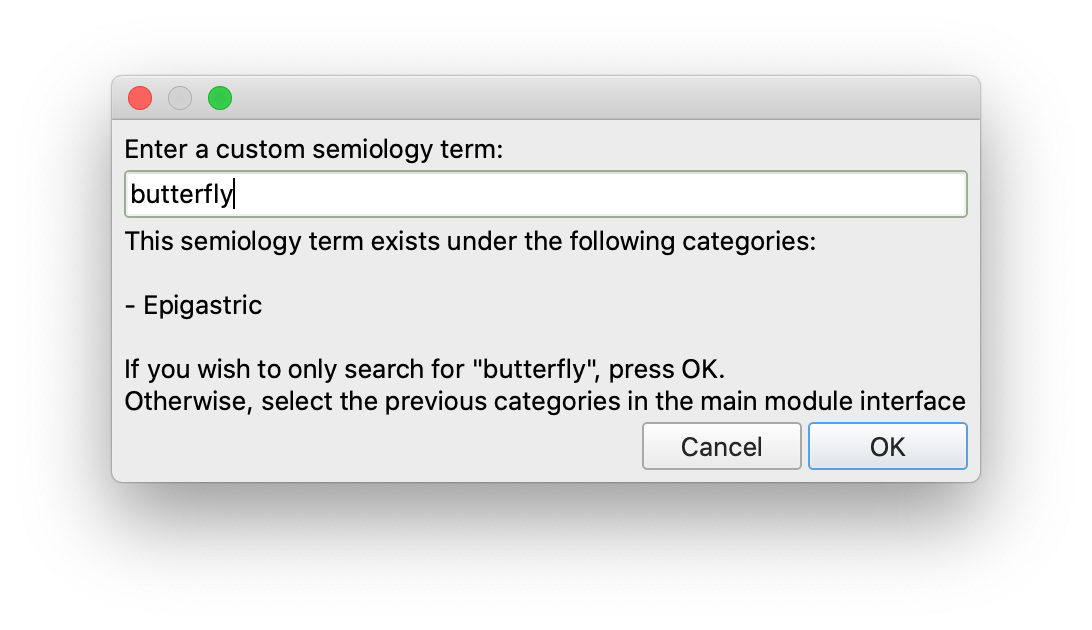
\includegraphics[width=\linewidth]{svt_custom}
  \caption[Adding a custom semiology term to the semiology visualization module]{
    Adding a custom semiology term to the semiology visualization module.
    In this case, the term \textit{butterfly} was entered as the patient described ``a butterfly feeling in my stomach''.
    The querying module matches the input term with the \textit{Epigastric} semiology term, and therefore the Slicer module suggests matching \textit{Epigastric} to the list of selected semiologies.
  }
  \label{fig:svt_custom}
\end{figure}


\subsection{Query}

The Slicer module reads the patient's semiologies and settings from the \ac{GUI} and generates a machine-readable query for the querying module.
As the waiting time to query the database is sometimes in the order of tens of seconds, previous queries result are cached in the disk for faster retrieval.
The result from querying the database is a table containing the number of datapoints for each brain structure (\cref{tab:single_semiology}).
If multiple semiologies are selected, results are combined and a number between 0 and 1 is computed for each brain structure by the querying module.
Details on how the datapoints are combined can be found in \cite{alim-marvasti_mapping_2021}.

The table is displayed on the \ac{GUI}, sorting the structures by number of datapoints, showing first the structures with the highest number of datapoints in the database (\cref{fig:svt_query}).

The probability map is generated and displayed, and the 2D slice views are centered on the brain structure with the highest number of associated datapoints.
Brain structures without datapoints are hidden from the 2D slice views and shown in gray on the 3D view.
To emphasize the importance of brain structures with a high number of datapoints, the opacity of each structure on the 2D slice views is linearly proportional to the number of associated datapoints.
We chose an open-source perceptually uniform sequential colormap, \textit{viridis}, as default for this application.
This implies that the brightness of each structure is also linearly proportional to the number of associated datapoints.
However, other colormaps are available if desired.
The colorbars on the 2D slice views help mapping colors to number of datapoints.

\begin{figure}
  \centering
  \svtscreenshot{svt_query}
  \caption[Results of querying the database with the \textit{Epigastric} semiology]{
    Results of querying the database with the \textit{Epigastric} semiology.
    Left: table showing the number of datapoints associated to each brain structure;
    right: \ac{EZ} probability map, where brightness (and opacity, on the 2D views) is linearly proportional to the number of datapoints.
  }
  \label{fig:svt_query}
\end{figure}


Advanced visualization settings may be selected, such as
showing only one hemisphere on the 3D view,
defining the minimum opacity on the 2D views or
enabling the color blind mode, in which the color-blind-friendly \textit{cividis} colormap is used \cite{nunez_optimizing_2018} (\cref{fig:svt_advanced}).

\begin{figure}
  \centering
  \svtscreenshot{svt_advanced}
  \caption[Demonstration of advanced visualization settings]{
    Demonstration of advanced visualization settings.
    The selected settings are:
    show only the right hemisphere,
    center the views on the right thalamus,
    set minimum opacity to 75\% (default is 25\%)
    and enable color-blind mode.
  }
  \label{fig:svt_advanced}
\end{figure}
